Il pattern architetturale applicato alla componente server è la \textit{Layered Architecture}. \\
Si è scelto tale pattern, sia perché lo si è ritenuto il più adatto a strutturare questo componente sia perchè, se la progettazione architetturale è stata fatta correttamente, i componenti del gruppo potranno lavorare su diversi layer autonomamente. Di seguito viene illustrato il diagramma dei package.
\begin{figure}[H]
	\centering
	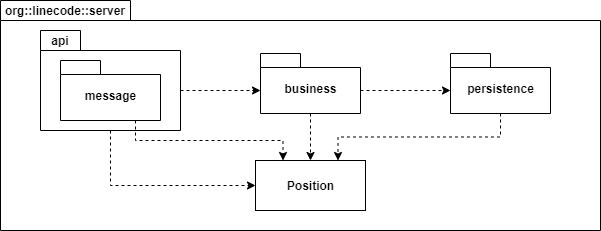
\includegraphics[width=12cm]{img/server_package.png}
	\caption{Server - Diagramma dei package}
\end{figure}

\subsubsection{Diagrammi delle classi}

\paragraph{Presentation layer}
Il server copre un ruolo centrale nell'applicazione, comunicando sia con le unità, che con l'interfaccia grafica. Qui infatti troviamo i metodi che permettono la gestione della connessione alle altre componenti del sistema, e quindi anche l'invio e la ricezione di messaggi. A tale scopo sono previste opportune interfacce.

\paragraph{Business layer}
Qui troviamo la logica per la gestione dei dati in entrata ed uscita dal server. \\
Per garantire l'indipendenza dal layer sovrastante, la comunicazione verrà implementata con un sistema di segnali e slot. Il business layer emetterà degli opportuni segnali che verranno intercettati dal layer sovrastante, ma la ricezione degli stessi non sarà di sua preoccupazione.

\paragraph{Persistence layer}
Per immagazzinare i dati  in uso all'applicazione, vengono utilizzate tre interfacce, per mappa, utenti ed unità, che vengono poi implementate in SQLite.

\paragraph{Database layer}
I dati che verranno immagazzinati nel database avranno la seguente struttura:
\begin{figure}[H]
	\centering
	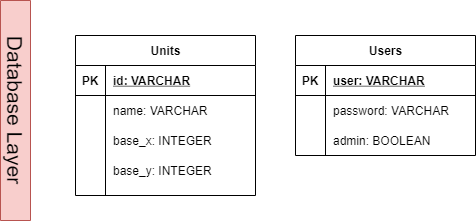
\includegraphics[width=8cm]{img/server_dblayer.png}
	\caption{Server - Database layer}
\end{figure}

\begin{landscape}
	\begin{figure}[h!]
		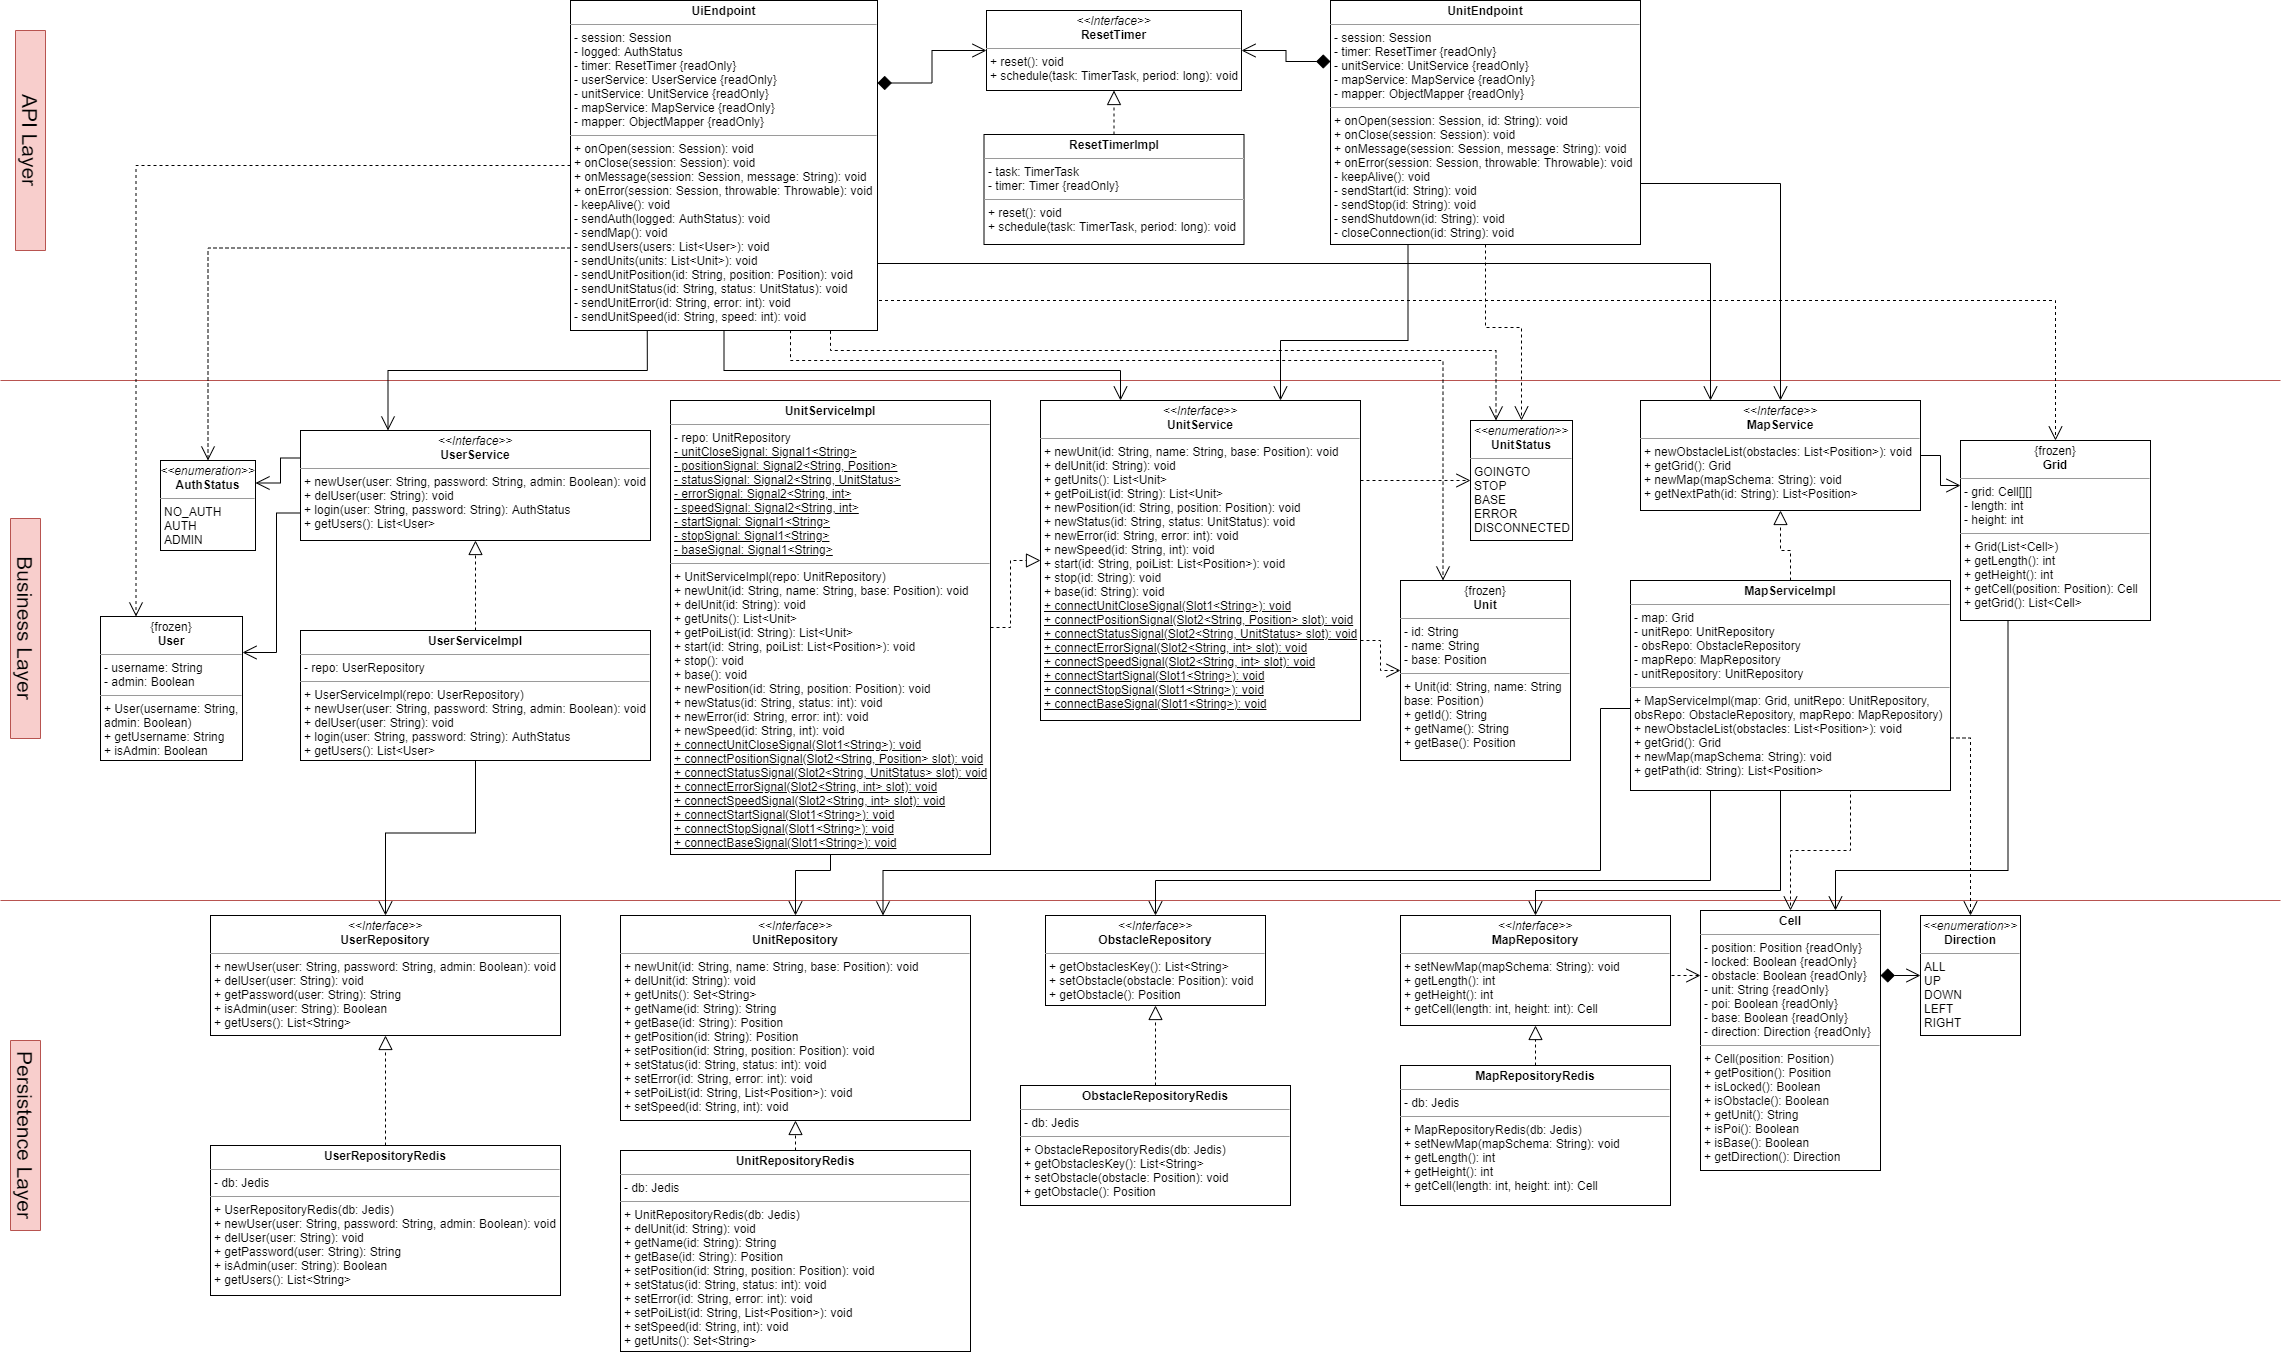
\includegraphics[width=24cm]{img/server_classi.png}
		\caption{Server - Diagramma delle classi}
	\end{figure}
\end{landscape}

\paragraph{Messages}
Per garantire i principi \textit{separation of concerns} e \textit{layer isolation}, sono state implementate delle interfacce allo scopo di essere gli oggetti di comunicazione tra i layer stessi.
\begin{figure}[H]
	\centering
	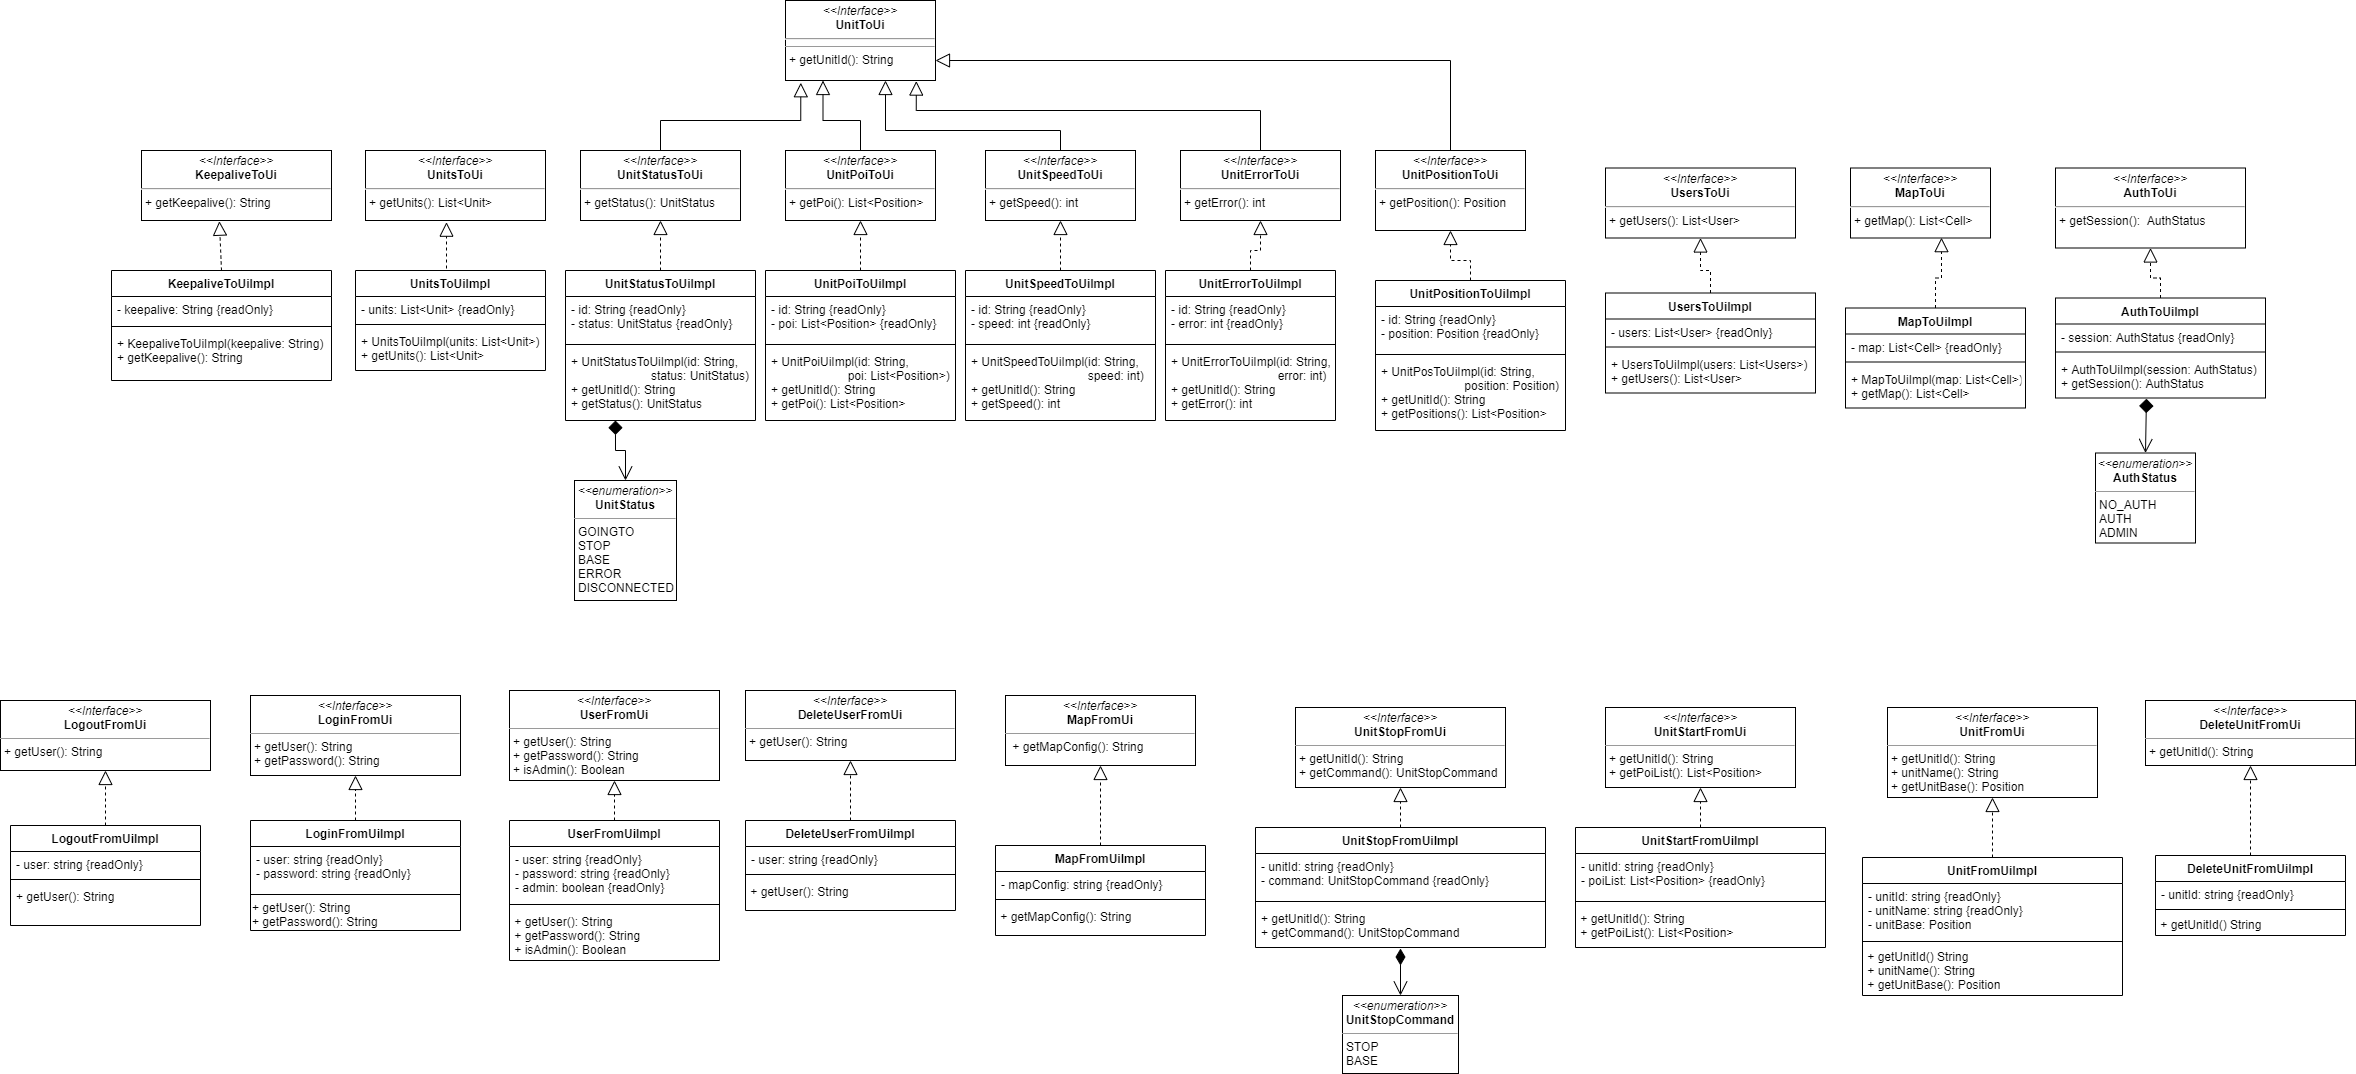
\includegraphics[width=18cm]{img/server_from_to_ui.png}
	\caption{Server - Messaggi da e per l'interfaccia}
\end{figure}
\begin{figure}[H]
	\centering
	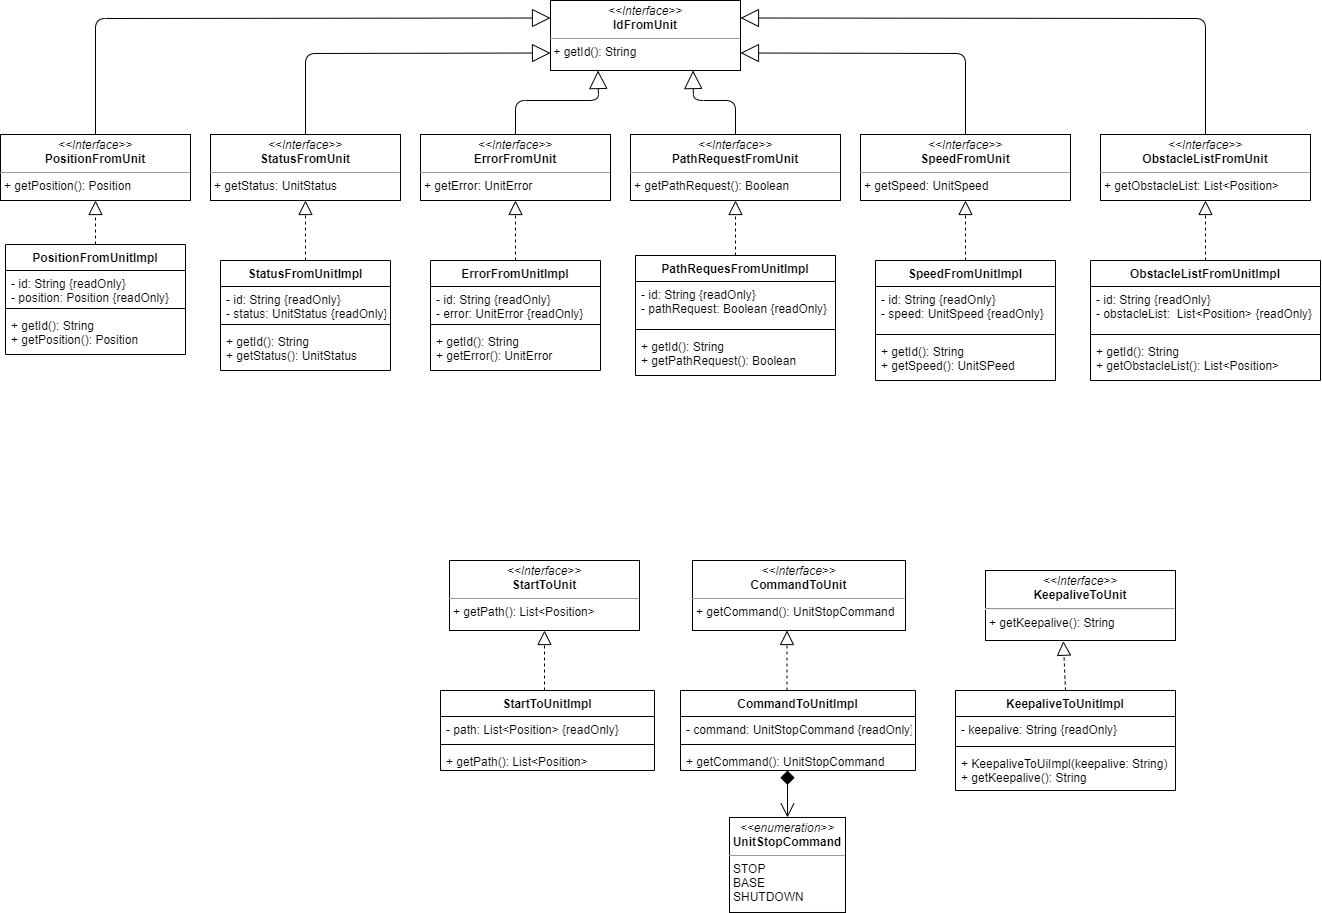
\includegraphics[width=18cm]{img/server_from_to_unit.png}
	\caption{Server - Messaggi da e per l'unità}
\end{figure}

\subsubsection{Diagrammi di sequenza}
Il seguente diagramma rappresenta il caso in cui l'interfaccia grafica invii al server una lista di \glock{POI}, che l'unità deve raggiungere.
\begin{figure}[H]
	\centering
	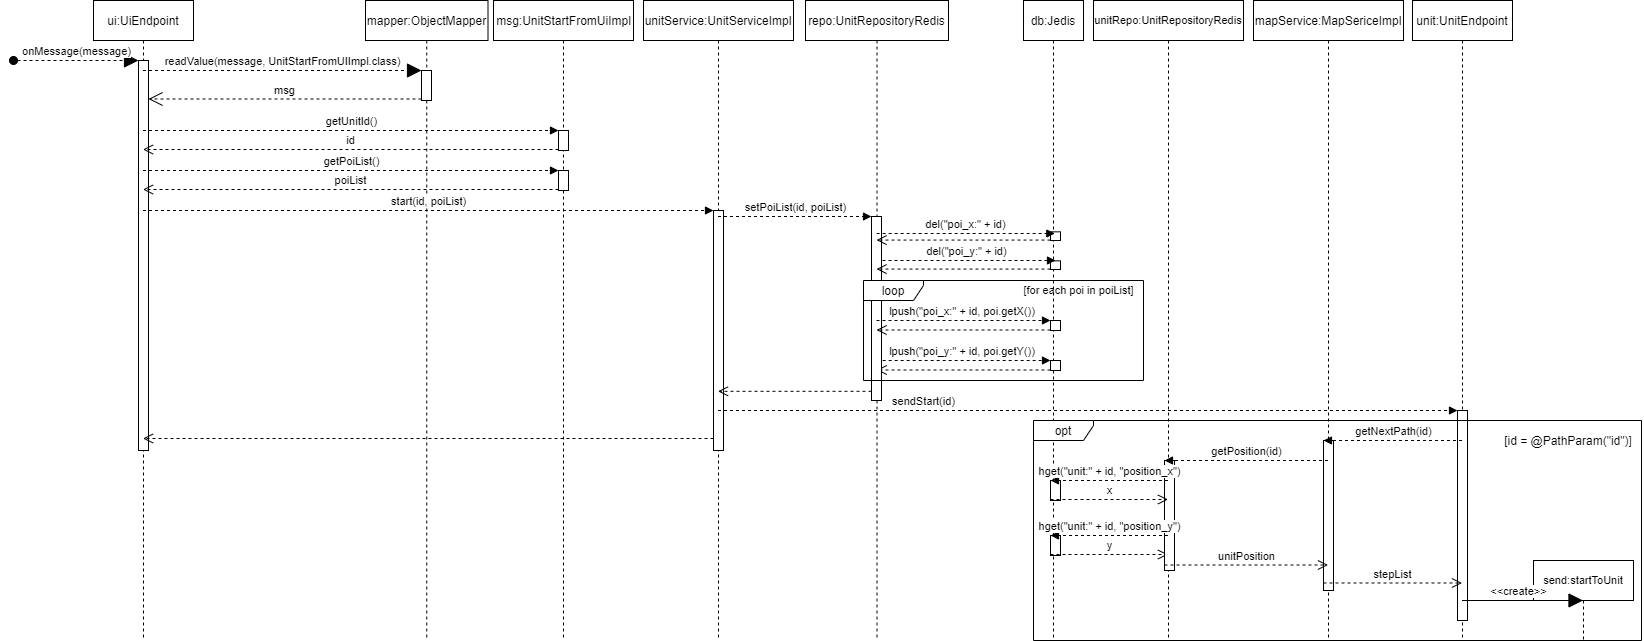
\includegraphics[width=13cm]{img/server_seq1.png}
	\caption{Server - Diagramma di sequenza}
\end{figure}

\newpage
Il seguente diagramma rappresenta il caso in cui un utente esegua il login dall'interfaccia grafica.
\begin{figure}[H]
	\centering
	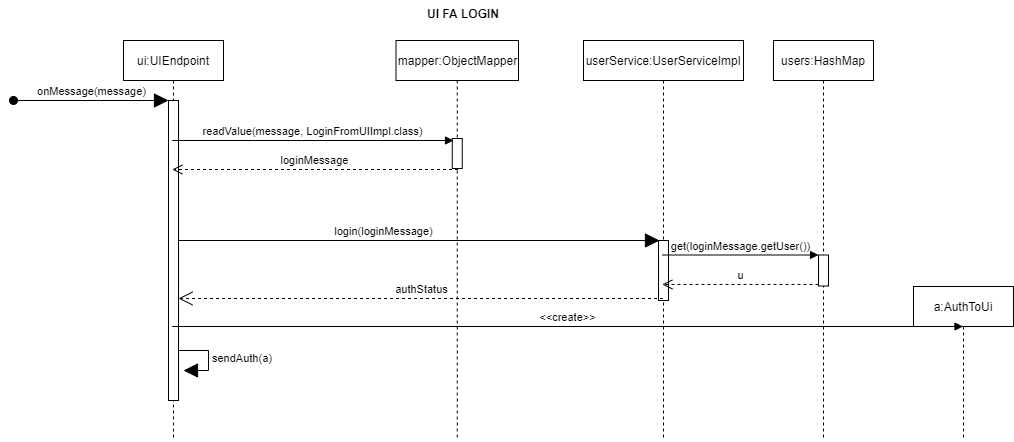
\includegraphics[width=13cm]{img/server_seq2.png}
	\caption{Server - Diagramma di sequenza}
\end{figure}

Il seguente diagramma rappresenta il caso in cui un utente elimini un'unità registrata.
\begin{figure}[H]
	\centering
	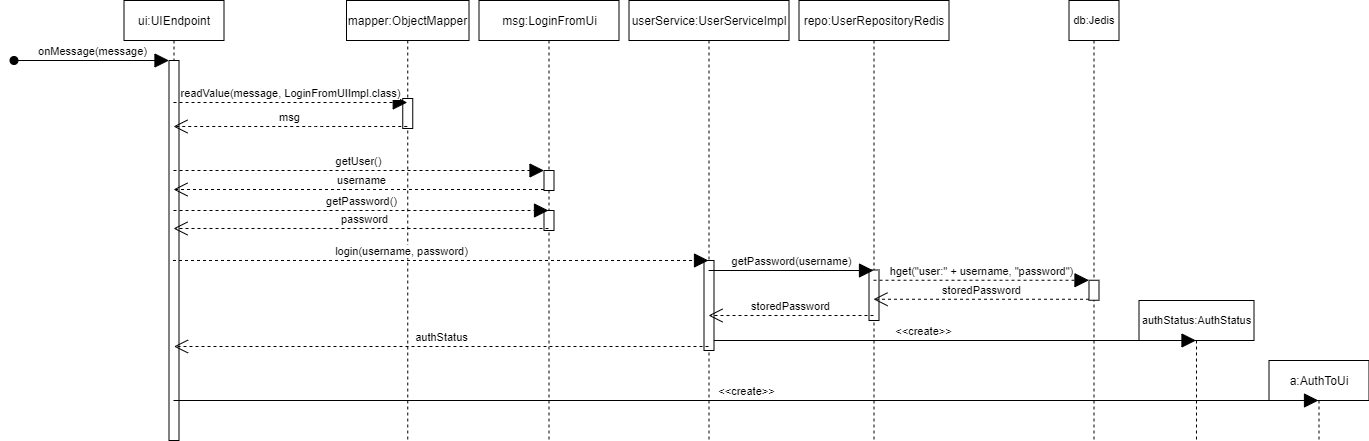
\includegraphics[width=13cm]{img/server_seq3.png}
	\caption{Server - Diagramma di sequenza}
\end{figure}